\documentclass[border=0.8ex,svgnames,tikz]{standalone}
\usepackage{amsmath,mathtools}
\usepackage{fontspec}
\setmainfont{Source Serif 4}
\setsansfont{Source Sans 3}
\setmonofont{Source Code Pro}

\usetikzlibrary{chains,calc}

\begin{document}
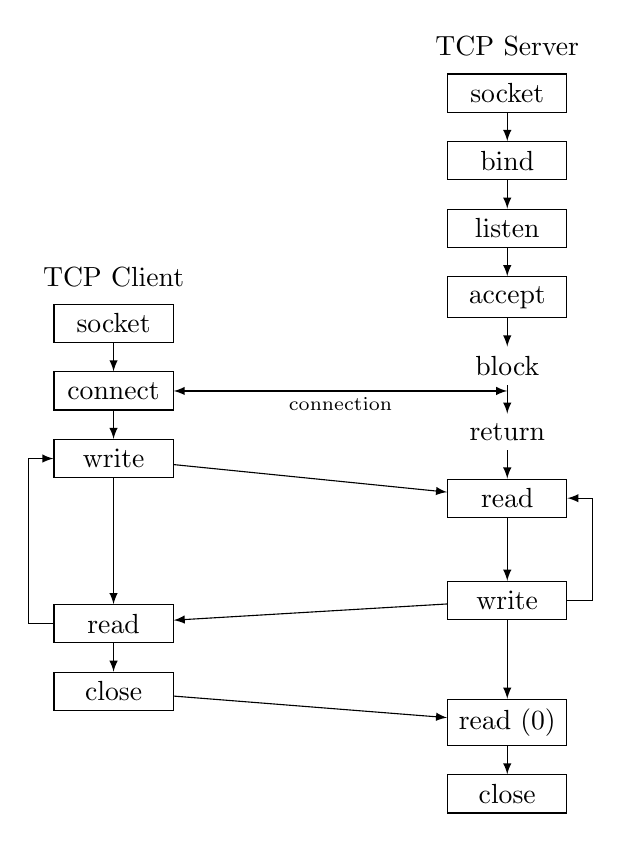
\begin{tikzpicture}[
  every label/.style={font=\scriptsize},
  function node/.style={
    draw,
    on chain,
    align=center,
    minimum width=10.0ex,
    minimum height=3.2ex,
    font=\normalsize,
  },
  every path/.style={draw,-latex},
  node distance=0.36,
  ]
  \begin{scope}[
    state node/.style={
      function node,
      draw=none,
      minimum height=0,
    },
    start chain=going below,
    every on chain/.style={join=by -latex},
    ]
    \node[function node] (server-socket) {socket};
    \node[function node] (server-bind)   {bind};
    \node[function node] (server-listen) {listen};
    \node[function node] (server-accept) {accept};
    \node[state node]    (server-block)  {block};
    \node[state node]    (server-return) {return};
    \node[function node] (server-read)   {read};
    \begin{scope}[node distance=0.8]
      \node[function node] (server-write) {write};
    \end{scope}
    \begin{scope}[node distance=1.0]
      \node[function node] (server-fin)  {read (0)};
    \end{scope}
    \node[function node] (server-close) {close};
  \end{scope}
  \begin{scope}[start chain=going below,every on chain/.style={join=by -latex}]
    \begin{scope}[node distance=0.35,every on chain/.style={}]
      \coordinate[on chain,left=5.0 of server-accept.north] (client-coor);
      \node[function node] (client-socket)  {socket};
    \end{scope}
    \node[function node] (client-connect) {connect};
    \node[function node] (client-write)   {write};
    \begin{scope}[node distance=1.6]
      \node[function node] (client-read) {read};
    \end{scope}
    \node[function node] (client-close) {close};
  \end{scope}
  \begin{scope}
    \node[draw=none,font=\normalsize,above=0.1 of server-socket] {TCP Server};
    \node[draw=none,font=\normalsize,above=0.1 of client-socket] {TCP Client};
    \path[latex-latex] (client-connect) -- node[inner
    sep=2pt,below,sloped,font=\scriptsize]{connection}
    ++($(server-accept.north)-(client-coor)$);
    \path (client-write) -- (server-read);
    \path (server-write) -- (client-read);
    \path (client-close) -- (server-fin);
    \path (server-write.east) -- ++(0.32,0) |- (server-read);
    \path (client-read.west) -- ++(-0.32,0) |- (client-write);
  \end{scope}
\end{tikzpicture}
\end{document}
